\subsection{Results}
For all trial runs a single environment was used. It consists of a 15 $\times$ 25 network with two stations and the following two agents:
\begin{verbatim}
train(0).
start(0,(6,19),0,w).
end(0,(10,5),63).
speed(0,1).
pow_type(0, electro).
weight(0,2).

train(1).
start(1,(9,5),0,e).
end(1,(7,19),63).
speed(1,1).
pow_type(1, diesel).
weight(1,1).

\end{verbatim}
\begin{figure}[htbp]
  \centering
  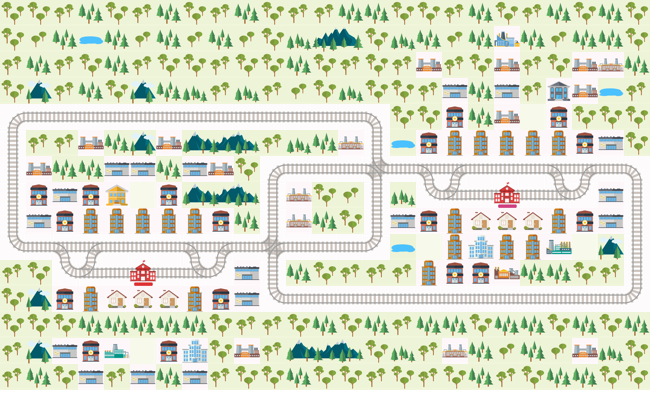
\includegraphics[width=0.8\textwidth]{./images/environment.png}
  \caption{Flatland environment used for all experiments}
  \label{fig:environment_image}
\end{figure}


The baseline encoding was only used to establish rules for bringing trains from a starting point to an end point with a proper behavior for a given environment. That goal was reached successfully: The baseline encoding successfully generated paths for all two agents from their starting point to their end points (see tables \ref{tab:baseline0} and \ref{tab:baseline1}) in a reasonable time frame of 16.029 seconds.

With the baseline routing established, we can analyze how the physical constraints of the energy encoding influence the trains' behavior. 

Train 0, defined as an electric train with a weight of 2, shows a significant acceleration on straight tracks. On straight tracks it reaches its maximum inverse speed of 1, which impacts its power consumption according to the squared speed formula. This causes energy spikes of 200 units per timestep. However, the solver strictly follows the turning constraints, forcing train 0 to slow down to an inverse speed of 3 before turning, such as the right turn at timestep 13 (see table \ref{tab:energy0}).

Train 1 is modeled as a diesel train with a weight of 1. This train's route showcases the regenerative braking capabilities defined in the encoding: When train 1 departs from a waiting state, it successfully regains a small amount of energy, logged as -7 units, at multiple intervals. It reaches its top inverse speed of 2, where its energy consumption peaks at 75 units on straight tracks (see table \ref{tab:energy1}).

The energy encoding managed to find a solution in 702.315 seconds, which is around 12 minutes. For this relatively small environment and two agents, this is unreasonable.